\documentclass[12pt]{article}

\usepackage{graphicx}
\usepackage{indentfirst}
\usepackage[utf8]{inputenc}
\usepackage{sbc-template}
\usepackage{url}
\usepackage{listings}

\lstset{language=[LaTeX]TeX,
        basicstyle=\ttfamily,
        columns=fullflexible,
        keepspaces=true}

\sloppy

\title{Relatório da Atividade Prática: DGEMM}
\author{Andrés Gonzalez Vilhena\\
        David Moreira Jacinto da Silva\\
        Lucas da Silva Inocencio}

\address{Escola Politécnica da Universidade Federal do Rio de Janeiro (UFRJ)\\
  Rio de Janeiro -- RJ -- Brasil
\email{agv1@poli.ufrj.br, davidmoreirajacinto.20222@poli.ufrj.br}
\email{lucas.inocencio@poli.ufrj.br}
}

\begin{document}

\maketitle

\begin{abstract}
    This document presents a comprehensive report on the optimization of the DGEMM operation. The investigation focuses on optimizing the DGEMM algorithm using various techniques, including vectorization, AVX instructions, loop unrolling, cache blocking, and parallelization with multiple threads. Python was used as the baseline for comparison, and the optimization was carried out using C and intrinsic functions. The results demonstrate significant performance improvements, achieving speedups of up to 4296.63 compared to the Python implementation. The study highlights the importance of leveraging hardware-specific features and optimization techniques to achieve efficient matrix multiplication on modern computing systems.
\end{abstract}

\section{Enunciado}

As operações com matrizes formam o núcleo dos códigos científicos que executam nos maiores supercomputadores do mundo, assim dado a relevância dos problemas estudados e os custos associados com a operação dessas grandes máquinas faz-se necessário que essas operações sejam executadas de maneira extremamente eficiente no hardware disponível. Em processadores de propósito geral essa eficiência somente é alcançada se o programador adaptar seus códigos aos recursos disponíveis na microarquitetura, reorganizando os padrões de acesso aos dados e fazendo uso de recursos especiais como instruções vetoriais.

Para essa tarefa um grupo de no máximo 3 alunos devem realizar uma investigação do código do DGEMM seguindo os passos indicados nas seções “Going Faster” do livro texto. O grupo deve realizar sua própria investigação de como as técnicas apresentadas melhoram o desempenho do DGEMM em suas plataformas. Cada grupo deve produzir um relatório descritivo a ser entregue no final do período (data especificada na página da disciplina), onde esse relatório deve conter uma explicação do problema DGEMM, além de uma seção para cada uma das otimizações feitas seguindo o que é apresentado em nossas aulas.

\section{Introdução}

O código-fonte está disponível em: \\
\url{https://github.com/lucas-inocencio/computer-architecture}

O problema de \textbf{D}ouble-\textbf{P}recision \textbf{Ge}neral \textbf{M}atrix \textbf{M}ultiply (DGEMM) é fundamental na área de Álgebra Linear, envolvendo o produto de matrizes de ponto flutuante de dupla precisão. Essa operação é amplamente utilizada em ciência da computação para resolver diversos problemas científicos. A multiplicação de matrizes é uma operação computacionalmente intensiva, especialmente para matrizes de grande porte, tornando a otimização do DGEMM essencial para alcançar alto desempenho em aplicações numéricas e científicas.

A forma geral do problema DGEMM pode ser expressa como:

\[ C = \alpha \cdot A \cdot B + \beta \cdot C \]

onde:

\begin{itemize}
    \item $A$, $B$ e $C$ são matrizes de dimensões adequadas (MxK, KxN e MxN, respectivamente).
    \item $\alpha$ e $\beta$ são valores escalares usados para a escala das matrizes $A \cdot B$ e $C$, respectivamente.
    \item O operador $\cdot$ representa a multiplicação de matriz.
\end{itemize}

Contudo, usaremos uma forma simplificada:

\[ C = A \cdot B \]

onde:

\begin{itemize}
    \item $A$, $B$ e $C$ são matrizes quadradas (NxN, NxN e NxN, respectivamente).
    \item O operador $\cdot$ representa a multiplicação matriz-matriz.
\end{itemize}


Especificacao da Maquina para os Testes:

\begin{itemize}
    \item AMD Ryzen 5 3400G
    \item 8GB RAM (Dual Channel)
    \item Windows 11 Pro 22H2
    \item GCC 13.1
    \item Python 3.11
\end{itemize}

\section{Desenvolvimento}

\subsection{Matrix Multiply in Python}

Para demonstrar o poder das ideias usaremos o codigo abaixo como base de comparacao para as otimizacoes.

Trecho de codigo original retirado do livro:

\begin{lstlisting}
    n = len(A)
    for i in range(n):
        for j in range(n):
            for k in range(n):
                C[i][j] += A[i][k] * B[k][j]
\end{lstlisting}

\begin{figure}[h]
    \centering
    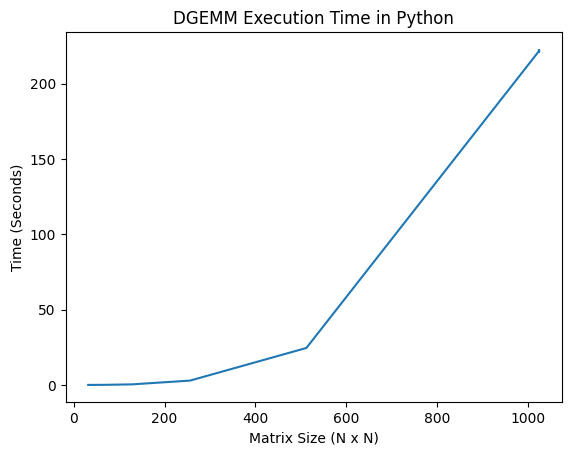
\includegraphics[scale=0.6]{figures/python.png}
    \caption{Python}
    \label{fig:python}
\end{figure}

\begin{table}[h]
    \centering
    \label{tab:python}
    \begin{tabular}{cccc}
        \textbf{size} & \textbf{time} & \textbf{std} \\
        32 & 0.005648 & 0.002063 \\
        64 & 0.048004 & 0.006445 \\
        128 & 0.366891 & 0.025504 \\
        256 & 2.873940 & 0.025432 \\
        512 & 24.524437 & 0.295540 \\
        1024 & 221.705985 & 1.308298 \\
    \end{tabular}
    \caption{Python}
\end{table}

Conforme mostrado na tabela de desempenho, mesmo para tamanhos de problemas relativamente pequenos, o Python exibe ineficiência na resolução de problemas de multiplicação de matrizes. Essa ineficiência se deve principalmente ao fato de o Python ser uma linguagem interpretada, o que normalmente resulta em uma execução mais lenta em comparação com as linguagens compiladas. Para tarefas computacionais intensivas, como multiplicação de matrizes, é recomendável usar linguagens compiladas ou utilizar bibliotecas otimizadas em Python (feitas em C), como NumPy ou Pandas, que podem melhorar significativamente o desempenho aproveitando otimizações e paralelização de baixo nível.

\subsection{Matrix Multiply in C}

Trecho de codigo original retirado do livro:


\begin{lstlisting}
    for (int i = 0; i < n; ++i)
        for (int j = 0; j < n; ++j)
        {
            double cij = C[i + j * n];
            for (int k = 0; k < n; k++)
                cij += A[i + k * n] * B[k + j * n];
            C[i + j * n] = cij;
        }
\end{lstlisting}

\begin{figure}[h]
    \centering
    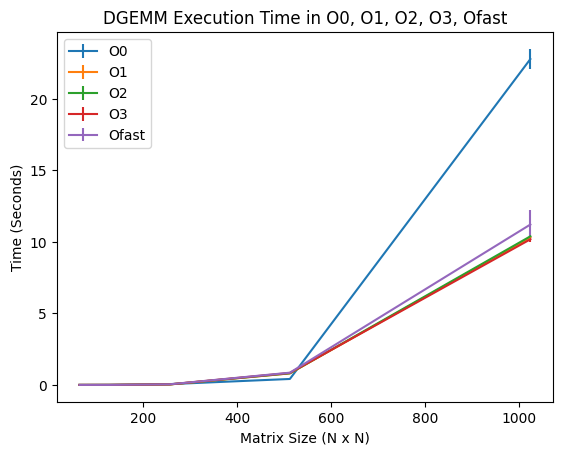
\includegraphics[scale=0.75]{figures/times_gcc.png}
    \caption{Times GCC Flags}
    \label{fig:times-gcc-flagsl}
\end{figure}

\begin{figure}[h]
    \centering
    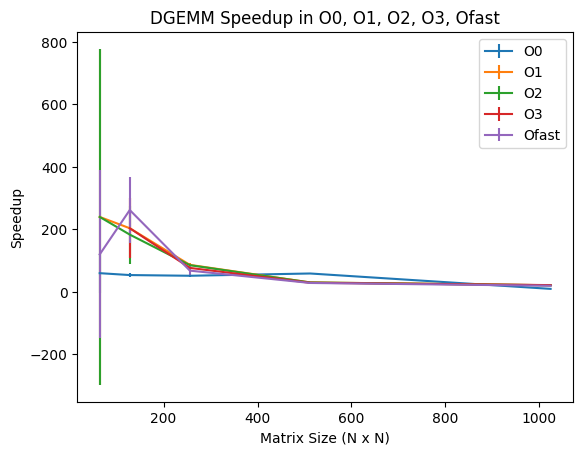
\includegraphics[scale=0.75]{figures/speedups_gcc.png}
    \caption{Speedups GCC Flags}
    \label{fig:speedups-gcc-flags}
\end{figure}

\begin{table}[h]
    \centering
    \label{tab:gcc-flags}
    \begin{tabular}{cccc}
        \textbf{flag} & \textbf{time} & \textbf{std speedup} & \textbf{speedup} \\
        Python & 221.705985 & 0.0 & 1\\
        O0 &	 22.786200   &	0.308210  &	9.729836 \\
        O1 & 10.307400 & 0.280380 & 21.509400 \\
        O2 & 10.390800 & 0.264848 & 21.336758 \\
        O3 & 10.182000 & 0.385060 & 21.774306 \\
        Ofast & 11.214800 & 1.825751 & 19.769054 \\
    \end{tabular}
    \caption{gcc flags}
\end{table}

É evidente que usar uma linguagem compilada como C e aproveitar a localidade espacial (dado que C armazena matrizes contíguas na memória) pode melhorar significativamente o desempenho da multiplicação de matrizes. Além disso, o uso de sinalizadores de otimização gcc apropriados aumenta ainda mais a velocidade de execução, com o sinalizador O3 demonstrando o melhor desempenho entre os sinalizadores testados.

\subsection{Subword Parallelism and Matrix Multiply}

Trecho de codigo original retirado do livro:

\begin{lstlisting}
    for (int i = 0; i < n; i += 4)
        for (int j = 0; j < n; j++)
        {
            __m256d c0 = _mm256_load_pd(C + i + j * n);
            for (int k = 0; k < n; k++)
                c0 = _mm256_add_pd(c0,
                     _mm256_mul_pd(_mm256_load_pd(A+i+k*n),
                     _mm256_set1_pd(B[k + j * n])));
            _mm256_store_pd(C + i + j * n, c0);
        }
    for (int i = 0; i < n; i += 4)
        for (int j = 0; j < n; j++)
        {
            __m256d c0 = _mm256_load_pd(C + i + j * n);
            for (int k = 0; k < n; k++)
                c0 = _mm256_add_pd(c0,
                     _mm256_mul_pd(_mm256_load_pd(A+i+k*n),
                     _mm256_broadcast_sd(B + k + j * n)));
            _mm256_store_pd(C + i + j * n, c0);
        }
\end{lstlisting}

A diferença entre o código original e o melhorado está no uso da função intrínseca mm256broadcastsd, que transmite o valor escalar B[k + j * n] para todos os elementos do registro AVX de 256 bits. Essa otimização reduz a necessidade de carregar o valor escalar várias vezes da memória durante o loop, melhorando o desempenho geral.

\begin{figure}[h]
    \centering
    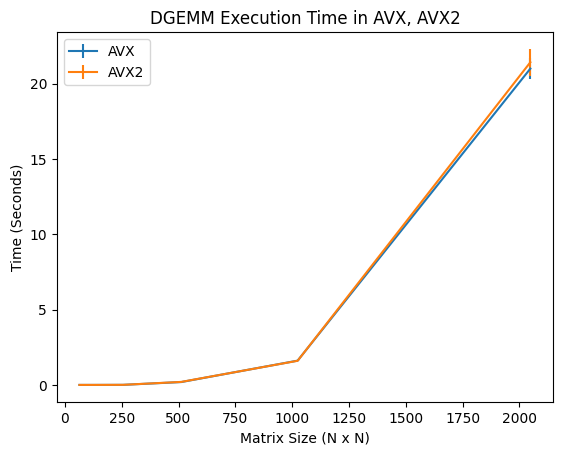
\includegraphics[scale=0.75]{figures/times_avx.png}
    \caption{Times AVX Instructions}
    \label{fig:times-avx}
\end{figure}

\begin{figure}[h]
    \centering
    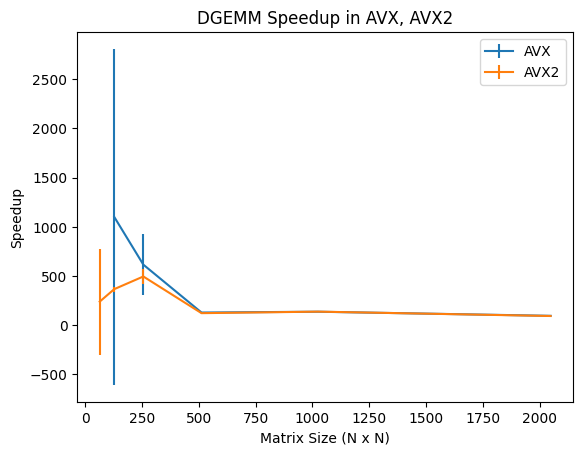
\includegraphics[scale=0.75]{figures/speedups_avx.png}
    \caption{Speedups AVX Instructions}
    \label{fig:speedups-avx}
\end{figure}

\begin{table}[h]
    \centering
    \label{tab:avx}
    \begin{tabular}{cccc}
        \textbf{Type} & \textbf{time} & \textbf{std speedup} & \textbf{speedup} \\
        None & 148.329424 & 1.825751 & 19.769054 \\
        AVX &	20.996636	 &	1.838429 &	137.563176\\
        AVX2 &	21.419500	 &	3.335001 &	138.375974\\
    \end{tabular}
    \caption{AVX}
\end{table}

demonstram a utilização do paralelismo de subpalavras usando instruções AVX (Advanced Vector Extensions) para multiplicação de matrizes. AVX é uma extensão de conjunto de instruções que permite o processamento de vários elementos de dados em paralelo, proporcionando melhorias significativas de desempenho para determinados cálculos.

\subsection{Instruction-Level Parallelism and Matrix Multiply}

Trecho de codigo original retirado do livro:

\begin{lstlisting}
    for (int i = 0; i < n; i += UNROLL * 4)
        for (int j = 0; j < n; ++j)
        {
            __m256d c[UNROLL];
            for (int r = 0; r < UNROLL; r++)
                c[r] = _mm256_load_pd(C + i + r * 4 + j * n);
    
            for (int k = 0; k < n; k++)
            {
                __m256d bb = _mm256_broadcast_sd(B + j * n + k);
                for (int r = 0; r < UNROLL; r++)
                    c[r] = _mm256_fmadd_pd(_mm256_load_pd(A+n*k+r*4+i), 
                                          bb, c[r]);
            }
            for (int r = 0; r < UNROLL; r++)
                _mm256_store_pd(C + i + r * 4 + j * n, c[r]);
        }
\end{lstlisting}

\begin{figure}[h]
    \centering
    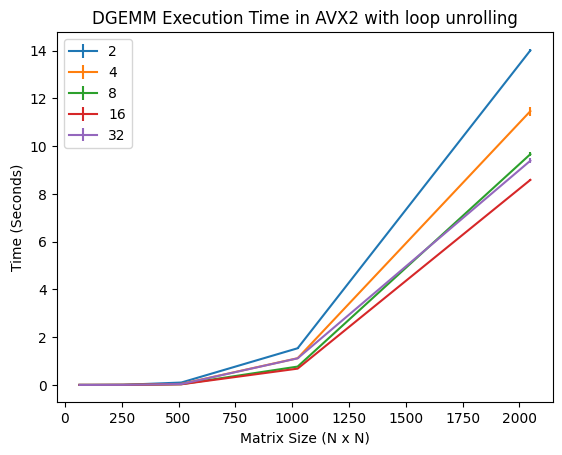
\includegraphics[scale=0.75]{figures/times_unroll.png}
    \caption{Times UNROLL}
    \label{fig:times-unroll}
\end{figure}

\begin{figure}[h]
    \centering
    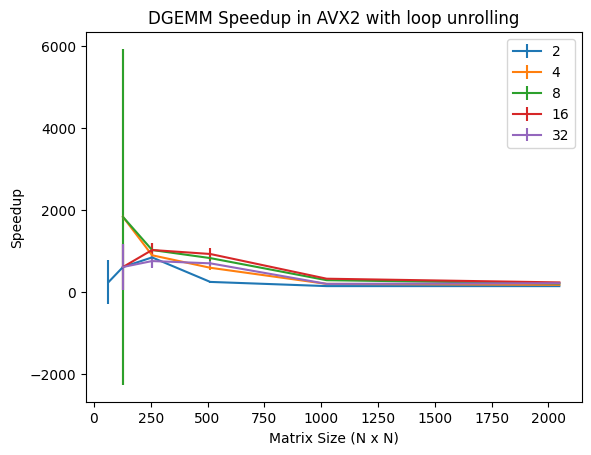
\includegraphics[scale=0.75]{figures/speedups_unroll.png}
    \caption{Speedups UNROLL}
    \label{fig:speedups-unroll}
\end{figure}

\begin{table}[h]
    \centering
    \label{tab:unroll}
    \begin{tabular}{cccc}
        \textbf{Num\_UNROLL} & \textbf{time} & \textbf{std speedup} & \textbf{speedup} \\
        1 & 21.419500 & 3.335001 & 138.375974 \\
        2 & 14.011400 & 3.475817 & 144.415050 \\
        4 & 11.466800 & 3.036342 & 198.270421 \\
        8 & 9.664400 & 3.251052 & 288.754864 \\
        16 & 8.587600 & 7.057091 & 325.082089 \\
        32 & 9.390600 & 2.875658 & 199.160964 \\
    \end{tabular}
    \caption{UNROLL}
\end{table}

\subsection{Cache Blocking and Matrix Multiply}

Trecho de codigo original retirado do livro:

\begin{lstlisting}
    void do_block(int n, int si, int sj, int sk, double *A, 
                double *B, double *C)
    {
        for (int i = si; i < si + BLOCKSIZE; ++i)
            for (int j = sj; j < sj + BLOCKSIZE; ++j)
            {
                double cij = C[i + j * n];
                for (int k = sk; k < sk + BLOCKSIZE; k++)
                    cij += A[i + k * n] * B[k + j * n];
                C[i + j * n] = cij;
            }
    }

    for (int sj = 0; sj < n; sj += BLOCKSIZE)
        for (int si = 0; si < n; si += BLOCKSIZE)
            for (int sk = 0; sk < n; sk += BLOCKSIZE)
                do_block(n, si, sj, sk, A, B, C);
\end{lstlisting}

\begin{figure}[h]
    \centering
    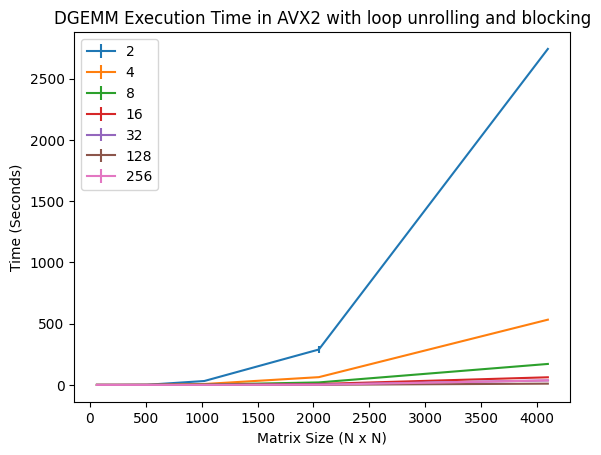
\includegraphics[scale=0.75]{figures/times_blocking.png}
    \caption{Times Blocking}
    \label{fig:times-blocking}
\end{figure}

\begin{figure}[h]
    \centering
    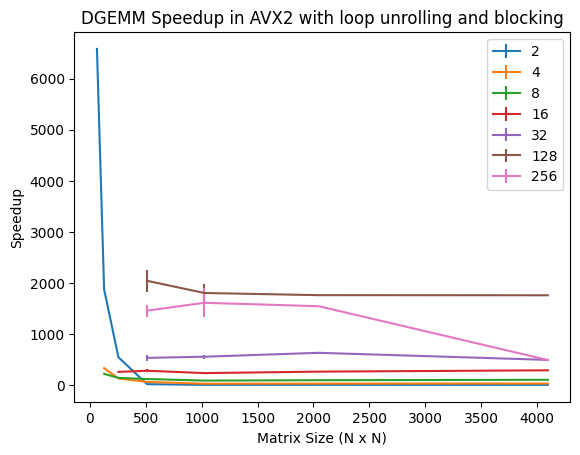
\includegraphics[scale=0.75]{figures/speedups_blocking.png}
    \caption{Speedups Blocking}
    \label{fig:speedups-blocking}
\end{figure}

\begin{table}[h]
    \centering
    \label{tab:blocking}
    \begin{tabular}{cccc}
        \textbf{blocksize} & \textbf{time} & \textbf{std speedup} & \textbf{speedup} \\
        2 & 2741.971699 & 0.753559	& 6.945720 \\
        4 & 532.456043 & 0.377248	&29.855371 \\
        8 & 171.177093	 & 0.851576	&90.967497 \\
        16 & 62.3320 & 5.452846	&237.728914 \\
        32 & 36.7116 & 41.334782	&558.172167 \\
        64 & 18.9454 & 106.366971&	1171.807531\\
        128 & 10.3458 & 180.797594&	1805.423330\\
        256 & 36.8776 & 285.966855&	1613.580676\\
    \end{tabular}
    \caption{Blocking}
\end{table}

\subsection{Multiple Processors and Matrix Multiply}

Trecho de codigo original retirado do livro:

\begin{lstlisting}
    void do_block(int n, int si, int sj, int sk,
                   double *A, double *B, double *C)
    {
        for (int i = si; i < si + BLOCKSIZE; i += UNROLL * 4)
            for (int j = sj; j < sj + BLOCKSIZE; j++)
            {
                __m256d c[UNROLL];
                for (int r = 0; r < UNROLL; r++)
                    c[r] = _mm256_load_pd(C + i + r * 4 + j * n);
                for (int k = sk; k < sk + BLOCKSIZE; k++)
                {
                    __m256d bb = _mm256_broadcast_sd(B + j * n + k);
                    for (int r = 0; r < UNROLL; r++)
                        c[r]=_mm256_fmadd_pd(_mm256_load_pd(A+n*k+r*4+i)
                                            , bb, c[r]);
                }
    
                for (int r = 0; r < UNROLL; r++)
                    _mm256_store_pd(C + i + r * 4 + j * n, c[r]);
            }
    }
\end{lstlisting}

\begin{lstlisting}
    omp_set_num_threads(P);
    #pragma omp parallel for
        for (int sj = 0; sj < n; sj += BLOCKSIZE)
            for (int si = 0; si < n; si += BLOCKSIZE)
                for (int sk = 0; sk < n; sk += BLOCKSIZE)
                    do_block(n, si, sj, sk, A, B, C);
\end{lstlisting}

\begin{figure}[h]
    \centering
    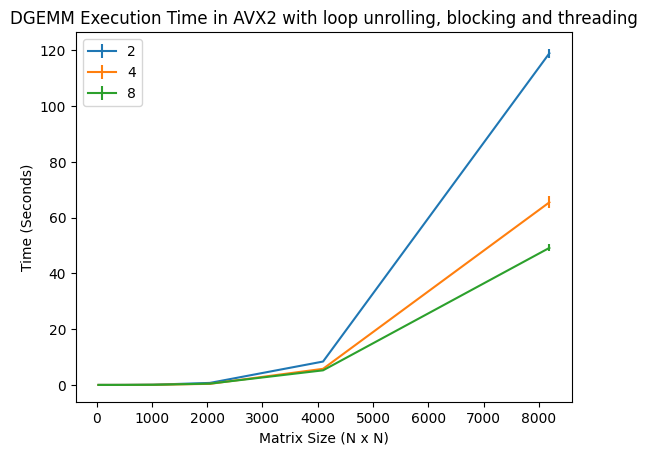
\includegraphics[scale=0.75]{figures/times_threads.png}
    \caption{Times Threads}
    \label{fig:times-threads}
\end{figure}

\begin{figure}[h]
    \centering
    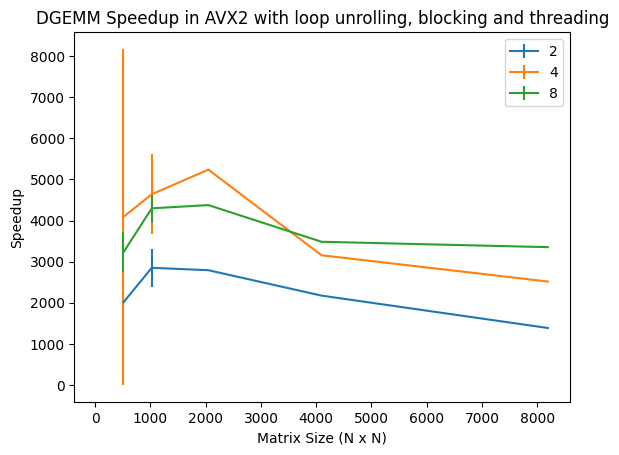
\includegraphics[scale=0.75]{figures/speedups_threads.png}
    \caption{Speedups Threads}
    \label{fig:speedups-threads}
\end{figure}

\begin{table}[h]
    \centering
    \label{tab:threads}
    \begin{tabular}{cccc}
        \textbf{threads} & \textbf{time} & \textbf{std speedup} & \textbf{speedup} \\
        1 & 319.6388 & 180.797594 & 1805.423330 \\
        2 & 118.9168 & 461.010250	& 2849.691322 \\
        4 & 65.4736 & 969.264761	& 4638.200520 \\
        8 & 49.1352	 & 	361.930530	& 4296.627614 \\
    \end{tabular}
    \caption{Threads}
\end{table}

A utilização de múltiplos processadores (ou threads) para realizar a multiplicação de matrizes em paralelo, usando a biblioteca OpenMP, demonstra um grande aumento no desempenho em relação à execução sequencial. O uso de 8 threads alcançou uma velocidade quase 6.5 vezes maior em comparação com o desempenho sequencial.

\section{Resultados}

\begin{figure}[h]
    \centering
    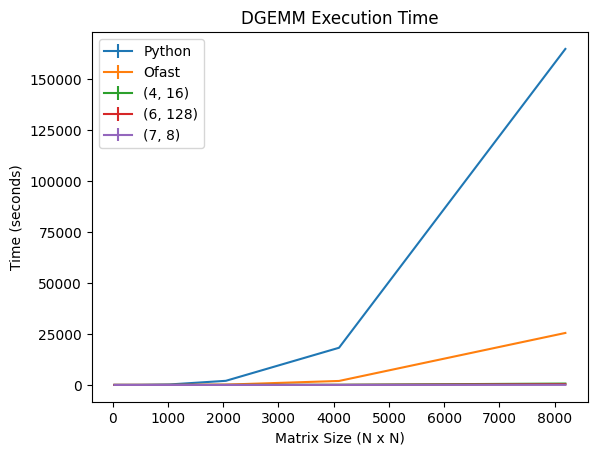
\includegraphics[scale=0.75]{figures/all_times_sizes.png}
    \caption{Comparação Final Tempos}
    \label{fig:times-finall}
\end{figure}

\begin{figure}[h]
    \centering
    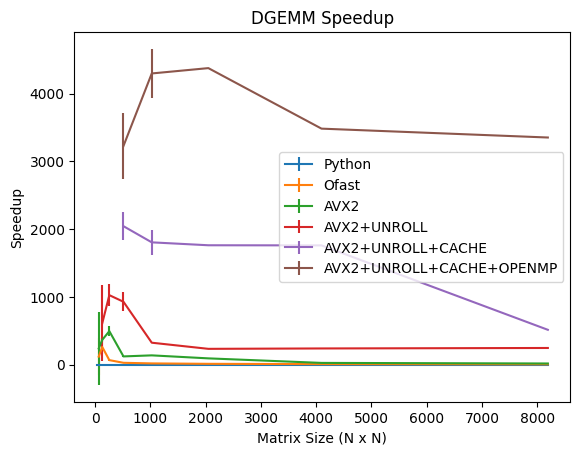
\includegraphics[scale=0.75]{figures/all_speedups_sizes.png}
    \caption{Comparação Final Speedups}
    \label{fig:speedups-final}
\end{figure}

\begin{table}[h]
    \centering
    \label{tab:final}
    \begin{tabular}{cccc}
        \textbf{Chapter} & \textbf{time} & \textbf{std speedup} & \textbf{speedup} \\
        1 & 164691.596770 & 0.0 & 1 \\
        2 & 25472.162249	 & 1.825751 &	19.769054 \\
        3 & 8877.037799 & 3.335001 &	138.375974 \\
        4 & 666.024234	 & 	7.057091	& 325.082089 \\
        5 & 319.6388	 & 	180.797594 &	1805.423330 \\
        6 & 49.1352	 & 	361.930530	& 4296.627614 \\
    \end{tabular}
    \caption{Comparação Final}
\end{table}

\section{Referências}

\begin{enumerate}
\item \textit{Computer Organization and Design RISC-V Edition: The Hardware Software Interface}, 2nd edition, by David A. Patterson and John L. Hennessy. Morgan Kaufmann, 2021.

\item \textit{Computer Organization and Architecture: Designing for Performance}, 11th edition, by William Stallings. Pearson, 2022.

\item \textit{Digital Design Using VHDL: A Systems Approach} by John F. Wakerly. Pearson, 2016.

\item Especificações AMD Ryzen 5 3400G retirado de \url{https://en.wikichip.org/wiki/amd/ryzen_5/3400g}

\item Microarquitetura Zen+ retirado de \url{https://en.wikichip.org/wiki/amd/microarchitectures/zen}

\item Documentação GCC retirado de \url{https://gcc.gnu.org/onlinedocs/gcc}

\end{enumerate}

\bibliography{sbc-template}

\end{document}